\section{Introduction and Goals}

According to the \acrfull{fao} in 2019, 931 millions tonne of food were wasted \cite{refart:FAOFW}. This has
environmental, but especially social consequences. In a world where approximately 9.9\% of the \cite{refart:AAHWH}
population suffers from hunger that waste percentage sounds paradoxal.

According to \acrfull{un} 5\% of the global food loss and waste comes from restaurants \cite{refart:UNSP}. 
The solution for this problem must be locally applied so its effects can be seen in a global structure. To do 
so we propose to develop a mobile application that connects restaurants, bakeries and or pastries to clients. The
former would offer their remaining products, which are still consumable, prior to the closing time, to a small price
and the latter would browser in the app to find which shops are offering products. 

We as ``Clean Up the World \textregistered'' are a rising StartUp whose main concerns is to find environmental solutions to
daily problems. Our portfolio includes projects about management of waste and optimization of household water 
usage. This product we want to develop targets small communities, like small cities or regions within a big city, 
to reduce the amount of wasted consumable food.

With our project we want to achieve the following goals:

\begin{itemize}
    \item Connect \glsplural{provider} with \glsplural{client}, so the former can offer products that the latter
    can purchase
    \item Collect statistical data about waste reduction within the \glsplural{provider}
    \item Promote reduction of food waste that still could be consumed
    \item Allow \glsplural{client} to have a different dining experience.
    \item Allow \glsplural{provider} to promote their products and gather new clients.
\end{itemize}

\subsection{Design Purpose}

The main purpose of this architecture is creating an exploratory prototype of an \gls{app}. We aim to test it with potential 
\glsplural{stakeholder} and regions to analyze their general acceptance and wishes \cite{refbook:DSHC} and get a fast feedback. 

This prototype will also make it feasible to identify unknown needs an wishes of the potential \glsplural{stakeholder}, so we 
can eventually increase the scope of functionality. Exploring this domain will also provide us with information regarding 
the behavior of our target group when it comes to buying and serving food that would be wasted, but is still consumable.

\subsection{Requirement Overview} \label{Requirement_Overview}

The following functionalities describe the basic requirement for the \gls{app}:

\begin{table}[H]
    \setstretch{1.0}
    \begin{tabularx}{\textwidth}{llX}
    \toprule
    Id & Requirement & Description  \\
    \midrule
    F-1 & Register as \gls{client}. & A \gls{client} can register to the app with its e-mail.\\
    F-2 & Login & After registration \gls{client} can login into the app. \\
    F-3 & Purchase option & A registered \gls{client} can purchase an available offer (see F7).\\
    F-4 & Filter/search options & A \gls{client} can perform filter and search actions for products.\\
    F-5 & Register as \gls{provider} & A \gls{provider} can register his store and add logos and pictures.\\
    F-6 & Create offer & A registered \gls{provider} can publishes what products they are offering with price 
    and amount. \\
    F-7 & Upload offer & A registered \gls{provider} can add, edit or remove offers to his catalog.\\
    F-8 & Check orders & A registered \gls{provider} can check all existing orders targeting his/her shops.\\
    \bottomrule
    \end{tabularx}
\end{table}

\begin{table}[H]
    \setstretch{1.0}
    \begin{tabularx}{\textwidth}{lX}
    \toprule
    ID & Motivation \\
    \midrule
    F-1 & The entry door of the \gls{app}, where our \gls{client} get an overview of all available offers \\
    F-2 & In order to place purchases our client need to be registered. It will also provide 
    statistical information about consumer behavior \\
    F-3 & Since we are dealing with a business relationship we have on one side a client willing to pay
    and for a product and on the other side a provider willing to offer a product/service \\
    F-4 & Like any other online-shop it is important that our \gls{client} can browse through the available possibilities\\
    F-5 & In order to make a product available a \gls{provider} needs to register his/her shop. This information will
    also be used for statistical analyzes about providers, products and consumer behavior \\
    F-6 - F-7 & A registered \gls{provider} can make an offer available according to his/her daily planning. 
    For future development of this app, this will be helpful to identify tendencies regarding dates, periods 
    and availabilities. \\
    F-8 & Also registered \glsplural{provider} can get an overview about how often their products have been sold. This
    may open a different kind of business orientation. \\
    \bottomrule
    \end{tabularx}
\end{table}

\newpage
The following \gls{use case diagram} displays an overview of the primary functionality of the app:

\begin{figure}[H]
    \centering
    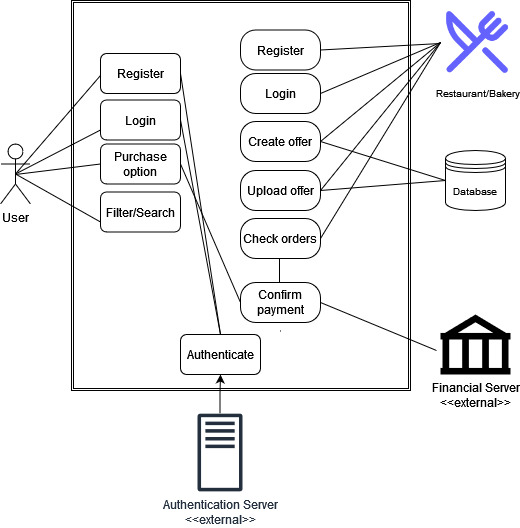
\includegraphics[width=0.5\textwidth]{assets/preliminary_functions.jpg}
    \caption{Preliminary functions}
    \label{fig:preliminary_use_case}
\end{figure}

\subsection{Qualitiy Goals}

The key qualities of this app are described in the table below:

\begin{table}[H]
    \setstretch{1.0}
    \begin{tabularx}{\textwidth}{|c|c|X|}
        \toprule
        \multicolumn{1}{c}{Quality} & \multicolumn{1}{c}{Priority} & \multicolumn{1}{c}{Motivation} \\
        \midrule
        \textbf{Usability} & 1 & Since we are working with a prototype it is important the usage is easy as possible,
        to attract more \glsplural{user} and to gather information about consumer behaviour. \glsplural{client} and \glsplural{provider}
        should have a simple interface where they can quickly interact without any burdens. \\
        \textbf{Interoperability} & 2 & To reduce programming burdens and accelerate the delivery of a working product the
        registration and payment process will rely on third party providers. For that reason the developed features should
        work faultless in combination with the external \acrfull{api}s (i.g \gls{mobile payment gateway} and \gls{federated login}). \\
        \textbf{Performance} & 3 & Many mobile and web-apps lose potential \glsplural{user} because of the lack of performance. A 
        \gls{system response} that takes too long (more than 1 second \cite{refonline:AP16M}) may frustrate potential \glsplural{user} 
        and discourage them of using the application. \\
        \bottomrule
    \end{tabularx}
\end{table}

\newpage

\subsection{Stakeholders} 

The main \glsplural{stakeholder} of this app are described in the table below:

\begin{table}[H]
    \setstretch{1.0}
    \begin{tabularx}{\textwidth}{lXX}
    \toprule
    Stakeholder & Description & Motivation  \\
    \midrule
    Providers & Owner of a restaurant, bakery or pastry. & One of the protagonist of this app. They will interact
    with clients using the app. From his usage we will gather valuable information about consumer behaviour. \\
    Clients & Person who wants to purchase last minute product from a provider. & The second protagonist of the app
    they will interact with the provider to search and to purchase product. The result of this interaction will
    provide us with statistical information to understand how food waste can be reduced.  \\
    Developers & Team in charge of creating the application using existing tactics and creating new solutions.
    & Responsable for guarantee that the main requirements of the app are fulfilled and fully functional. 
    Since they will be dealing with the background of the product, it is important that they understand it very
    good so it can also be implemented in a final version.\\
    Boarding Committee of \\ ``Clean Up the Word (R)'' & Members of the management team who wants to delivery 
    environmental solution do daily problems and at the same time develop a profitable product.
    & Group in charge of main decisions regarding what will be developed. Their decision are based on mark tendencies
    and on environmental issues.  \\
    Environment Activist & Part of the society who aims to find environmental solutions to daily problems.
    & They integrate local discussion groups, local public institutions, schools and universities. 
    They are the one who brings their concerns to the boarding committee. \\
    \bottomrule
    \end{tabularx}
\end{table}